\documentclass[compress]{beamer}
\usetheme{CambridgeUS}
\usefonttheme{serif}
\usecolortheme{dove}
\useinnertheme{rounded}
\useoutertheme{miniframes}
\usepackage{graphicx}
\usepackage{setspace}
\usepackage{tabularx}
\usepackage{tikzsymbols}
\usepackage{tikz}
\usepackage{spot}
\usepackage[italian]{babel}
\usepackage{tabularx}
\usepackage[absolute,overlay]{textpos}
\usepackage{booktabs}
\usepackage{fancyvrb}
\usepackage{xcolor}
\usepackage{multicol}
\usepackage{multirow}
\usepackage{listings}

\lstset{language=R,%
	basicstyle=\ttfamily\small,%
	%commentstyle=\slshape\color{gray},%
	commentstyle=\color{gray},%
	basewidth={.49em, .4em},%
	showstringspaces=false,%
	emphstyle=\color{red}}


\newcommand\Factor{1.2}
\definecolor{unipd}{RGB}{155, 0, 20}
\definecolor{grigioPantano}{RGB}{72,79,89}


\setbeamerfont{block title}{family=\bfseries}
\setbeamercolor{block title}{use=structure,fg=unipd,bg=white}

%\setbeamertemplate{footline}[page number]
\setbeamerfont{subtitle}{size=\large, series=\bfseries}
\definecolor{template}{RGB}{54, 114, 89}
\definecolor{background}{RGB}{250, 250, 250}
\definecolor{royalblue3}{RGB}{58,95,205}
\definecolor{giallo}{RGB}{197, 151, 0}
\definecolor{blu}{RGB}{19 101 158}
\setbeamercolor{frametitle}{fg=template, bg=white}
\setbeamercolor{section in head/foot}{bg=template, fg=template!20}
\setbeamercolor{subsection in head/foot}{bg=template!20, fg=template}
\setbeamercolor{author in head/foot}{bg=template, fg=template!20}
\setbeamercolor{date in head/foot}{bg=template, fg=white}
\setbeamercolor{page number in head/foot}{bg=template, fg=white}
\setbeamercolor{title in head/foot}{fg=template}
\setbeamercolor*{item}{fg=template}
\setbeamertemplate{frametitle}{\color{template}\bfseries\scshape\insertframetitle\par\hrulefill}
\setbeamercolor{title}{fg=template}
\definecolor{unipd}{RGB}{155, 0, 20}
\definecolor{highlight}{RGB}{54, 114, 89}
\definecolor{back}{RGB}{247, 251, 255}
\definecolor{map}{RGB}{111, 172, 232}
\definecolor{childmap}{RGB}{161, 200, 240}
\definecolor{nodemap}{RGB}{141, 170, 199}
\definecolor{rasch}{rgb}{0.0, 0.33, 0.71}
\definecolor{log}{rgb}{0.0, 0.65, 0.58}
\definecolor{diff}{RGB}{33, 113, 181}
\definecolor{single}{RGB}{106, 81, 163}
\definecolor{comp}{RGB}{35, 99, 70}
\definecolor{inc}{RGB}{191, 13, 43}
\definecolor{highlight}{rgb}{0.45, 0.31, 0.59}
\definecolor{section}{RGB}{51,51,179}
\definecolor{typical}{RGB}{8, 69, 148}
\definecolor{model}{RGB}{74, 20, 134}
\definecolor{orangered2}{RGB}{238,64,0}
\definecolor{royalblue3}{RGB}{58,95,205}
\definecolor{springgreen}{RGB}{0,205,102}
\definecolor{magenta}{RGB}{255,0,255}

  \tikzset{
	invisible/.style={opacity=0},
	visible on/.style={alt={#1{}{invisible}}},
	alt/.code args={<#1>#2#3}{%
		\alt<#1>{\pgfkeysalso{#2}}{\pgfkeysalso{#3}} % \pgfkeysalso doesn't change the path
	},
	every overlay node/.style={
		%draw=black,fill=white,rounded corners,
		anchor=north west, inner sep=0pt,
	},
}

\usetikzlibrary{shapes.geometric, arrows}
\tikzstyle{respondent} = [rectangle, minimum width=1.5cm, minimum height=1cm,text centered, draw=white]
\tikzstyle{stimulus} = [rectangle, minimum width=1.5cm, minimum height=1cm,text centered, draw=white]
\tikzstyle{trial} = [rectangle, minimum width=1cm, minimum height=1cm,text centered, draw=black]
\tikzstyle{process} = [rectangle, rounded corners, minimum width=0.5cm, minimum height=1cm, text width =2.5cm, text centered, draw=black]
\tikzstyle{arrow} = [thick,->,>=stealth]
\tikzstyle{condition} = [rectangle, rounded corners,draw=black,text width=2cm, text height=6.5cm]
\tikzstyle{latent} = [ellipse, minimum width=2.5cm, minimum height=2cm,text centered, draw=black]
\tikzstyle{item} = [rectangle, rounded corners, minimum width=0.5cm, minimum height=1cm, text width =1.5cm, text centered, draw=black]
\tikzstyle{arrow} = [thick,->,>=stealth]

\def\tikzoverlay{%
	\tikz[remember picture, overlay]\node[every overlay node]
}%


\AtBeginSection[]
{
	\begin{frame}
		\tableofcontents[currentsection,currentsubsection]
	\end{frame}
}  



%\title[Implicit assessment]{Implicit assessment in psychology: \\ How to work with the IAT}
\title[Misurazione implicita]{Misurazione Implicita in Psicologia: \\ Un approccio diverso per l'analisi dei dati IAT}
\date[PSQT, 2024]{Master di II Livello \\ Psicologia quantitativa: Misurazione, valutazione e analisi di variabili psicosociali }
\institute[]{18 luglio 2024, Padova}
\author[Ottavia M. Epifania]{\texorpdfstring{Ottavia M. Epifania, Ph.D.\newline\url{ottavia.epifania@unipd.it}}{Author}}

\begin{document}
	\tikzstyle{every picture}+=[remember picture]
	


\begin{frame}[plain]
    \maketitle
\end{frame}




\section{Look at the data!}

\begin{frame}
	\centering
	\scalebox{.50}{
		\begin{tikzpicture}[inner sep=1pt,auto=left, node distance=2cm,>=latex']
			
			\node(s1) at(2, 16)  [respondent]  {$p_1$};
			\node(s2) at (2, 11) [respondent] {$p_2$};
			\node(s3) at (2, 5.5) [respondent] {$p_3$};
			\node(t1) at (12, 17) [ trial] {};
			\node(t2) at (12, 15.5) [trial] {};
			\node(t3) at (12, 14) [trial] {};
			\node(t4) at (12, 12.5) [trial] {};
			\node(t5) at (12, 9) [trial] {};
			\node(t6) at (12, 7.5) [trial] {};
			\node(t7) at (12, 6) [trial] {};
			\node(t8) at (12, 4.5) [trial] {};
			\node(stim1) at(22, 13)  [stimulus]  {\Smiley[3]};
			\node(stim2) at (22, 7) [stimulus] {\Sleepey[3]};
			\node at (12, 14.8) [condition, dashed,ultra thick] {};  
			\node at (12, 6.8) [condition, black,ultra thick] {};  
			\draw [->, shorten >= +3pt] (s1.east) -- (t1.west);
			\draw [->, shorten >= +3pt] (s2.east) -- (t1.west);
			\draw [->, shorten >= +3pt] (s3.east) -- (t1.west);
			\draw [->, shorten >= +3pt] (s1.east) -- (t2.west);
			\draw [->, shorten >= +3pt] (s2.east) -- (t2.west);
			\draw [->, shorten >= +3pt] (s3.east) -- (t2.west);
			\draw [->, shorten >= +3pt] (s1.east) -- (t3.west);
			\draw [->, shorten >= +3pt] (s2.east) -- (t3.west);
			\draw [->, shorten >= +3pt] (s3.east) -- (t3.west);
			\draw [->, shorten >= +3pt] (s1.east) -- (t4.west);
			\draw [->, shorten >= +3pt] (s2.east) -- (t4.west);
			\draw [->, shorten >= +3pt] (s3.east) -- (t4.west);
			\draw [->, shorten >= +3pt] (s1.east) -- (t5.west);
			\draw [->, shorten >= +3pt] (s2.east) -- (t5.west);
			\draw [->, shorten >= +3pt] (s3.east) -- (t5.west);
			\draw [->, shorten >= +3pt] (s1.east) -- (t6.west);
			\draw [->, shorten >= +3pt] (s2.east) -- (t6.west);
			\draw [->, shorten >= +3pt] (s3.east) -- (t6.west);
			\draw [->, shorten >= +3pt] (s1.east) -- (t7.west);
			\draw [->, shorten >= +3pt] (s2.east) -- (t7.west);
			\draw [->, shorten >= +3pt] (s3.east) -- (t7.west);
			\draw [->, shorten >= +3pt] (s1.east) -- (t8.west);
			\draw [->, shorten >= +3pt] (s2.east) -- (t8.west);
			\draw [->, shorten >= +3pt] (s3.east) -- (t8.west);
			\draw [<-, shorten <= +3pt] (t1.east)  -- (stim1.west); 
			\draw [<-, shorten <= +3pt] (t2.east)  -- (stim2.west); 
			\draw [<-, shorten <= +3pt] (t3.east)  -- (stim1.west); 
			\draw [<-, shorten <= +3pt] (t4.east)  -- (stim2.west); 
			\draw [<-, shorten <= +3pt] (t5.east)  -- (stim1.west); 
			\draw [<-, shorten <= +3pt] (t6.east)  -- (stim2.west); 
			\draw [<-, shorten <= +3pt] (t7.east)  -- (stim1.west); 
			\draw [<-, shorten <= +3pt] (t8.east)  -- (stim2.west); 
		\end{tikzpicture}
	}
	
\end{frame}




\begin{frame}
	
	\begin{block}{I rispondenti sono fattori random}
		
		Campione prelevato da una popolazione più ampia
		
		\vspace{1.5mm}

		È necessario riconoscere la variabilità del campionamento
		
		\vspace{1.5mm}
		I risultati possono essere generalizzati ad altri rispondenti appartenenti alla stessa popolazione
	\end{block}
	
	\vspace{3mm}
	\pause
	\begin{block}{Gli stimoli sono fattori fissi}
		
		Presi come intera popolazione
		
		\vspace{1.5mm}
		Non c'è variabilità del campionamento
		
		\vspace{1.5mm}
		
		Non è necessario generalizzare i risultati perché gli stimoli sono la popolazione
		
	\end{block}
\end{frame}

\begin{frame}	
	Gli stimoli sono un campione delle rispettive categorie di appartenenza: 
	
	\footnotesize
	
	
	\begin{block}{12 stimuli delle categorie target}
		\begin{columns}
			\column{.50\linewidth}
			\centering
			Volti di persone Bianche
			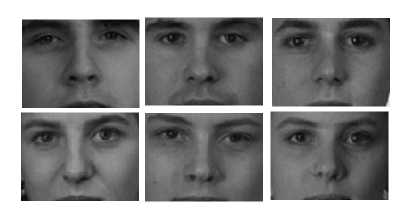
\includegraphics[width=\linewidth]{img/white.png}
			
			\column{.50\linewidth}
			\centering
		Volti di persone Nere
			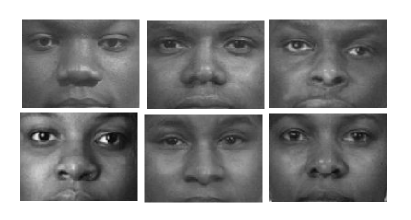
\includegraphics[width=\linewidth]{img/black.png}
		\end{columns}		
	\end{block}
	
	
	
	\begin{block}{16 stimuli attributo}
		
		\begin{columns}[T]
			\begin{column}{.50\linewidth}
				\begin{center}
					\color{rasch} Attributi positivi
				\end{center}
				
				Good, laughter, pleasure, glory, peace, happy, joy, love
			\end{column}
			
			\begin{column}{.50\linewidth}
				\begin{center}
					\color{alert}Attributi negativi
				\end{center}
				
				Evil, bad, horrible, terrible, nasty, pain, failure, hate
			\end{column}
		\end{columns}
	\end{block}
\end{frame}

\begin{frame}{}
	
	\begin{block}{Generalizzabilità}
		
		\small
		
		La generalizzabilità è limitata al set specifico di stimoli utilizzato nell'esperimento
		
		I risultati possono essere generalizzati se e solo se viene utilizzato esattamente lo stesso set di stimoli
		
		
	\end{block}
	
	\pause
	
	\begin{block}{Robustezza dei risultati}
		
		\small
		La variabilità casuale a livello degli stimoli potrebbe aumentare la probabilità di commettere errori di Tipo I
		
		La media degli stimoli per ottenere punteggi a livello di persona porta a stime distorte a causa del rumore nei dati
	\end{block}
	
	\pause
	
	\begin{block}{Perdita di informazione}
		
		\small
		
		Non viene considerata tutta la variabilità né tutte le informazioni che possono essere ottenute da essa
		
		Ogni stimolo è considerato come se fosse ugualmente informativo
	\end{block}
	
\end{frame}

\section{Una possibile soluzione}

\begin{frame}{The supermodel(s)}
	\vskip0pt plus 1filll
	\begin{center}
		\Large{\textbf{Linear Mixed-Effects Models}} (LMMs)
	\end{center}
	
	\vspace{5mm}
	\begin{itemize}
		\item[{\small
\includegraphics[height=3ex]{supergirl.png}}] Considerare (potenzialmente) tutte le fonti di variabilità e dipendenza nei dati
		\vspace{1.5mm}
		\item[{\small
\includegraphics[height=3ex]{supergirl.png}}] Raccogliere informazioni a livello del singolo stimolo
		\vspace{1.5mm}
		\item[{\small
\includegraphics[height=3ex]{supergirl.png}}] Ottenere stime di tipo Rasch
	\end{itemize}
	\vskip0pt plus 1filll
	
	\color{template}\rule{0.30\linewidth}{0.5pt}\\
	\color{black}
	\footnotesize{Epifania, O. M., Robusto, E., \& Anselmi, P. (2021). Rasch gone mixed: A mixed model approach to
		the Implicit Association Test. \emph{Testing, Psychometrics, Methodology in Applied Psychology,
			28}, 467–483. doi: 10.4473/TPM28.4.5}
\end{frame}


\begin{frame}{Effetti e fattori random}
	
	Combinazione lineare dei predittori in un modello lineare:
	\begin{equation*}
		\eta = X \beta,
	\end{equation*}
	dove $\beta$ indica i coefficienti dell'intercetta fissa e della(e) pendenza(e) fissa, e $X$ è la matrice del modello.
	
	
	Combinazione lineare dei predittori in un modello lineare ad effetti misti (LMM):
	
	\begin{equation*}
		\eta = X \beta + Zd,
	\end{equation*}
	dove $Z$ è la matrice e $d$ è il vettore degli effetti casuali (non parametri!)
	
	
	\vspace{2.5mm}
	\begin{center}
		\emph{Best Linear Unbiased Predictors}
	\end{center}
\end{frame}


\begin{frame}{Modelli Generalizzati Lineari (GLM) per risposte dicomtomiche}
	
	\begin{figure}
		\begin{overprint}
			\onslide<1>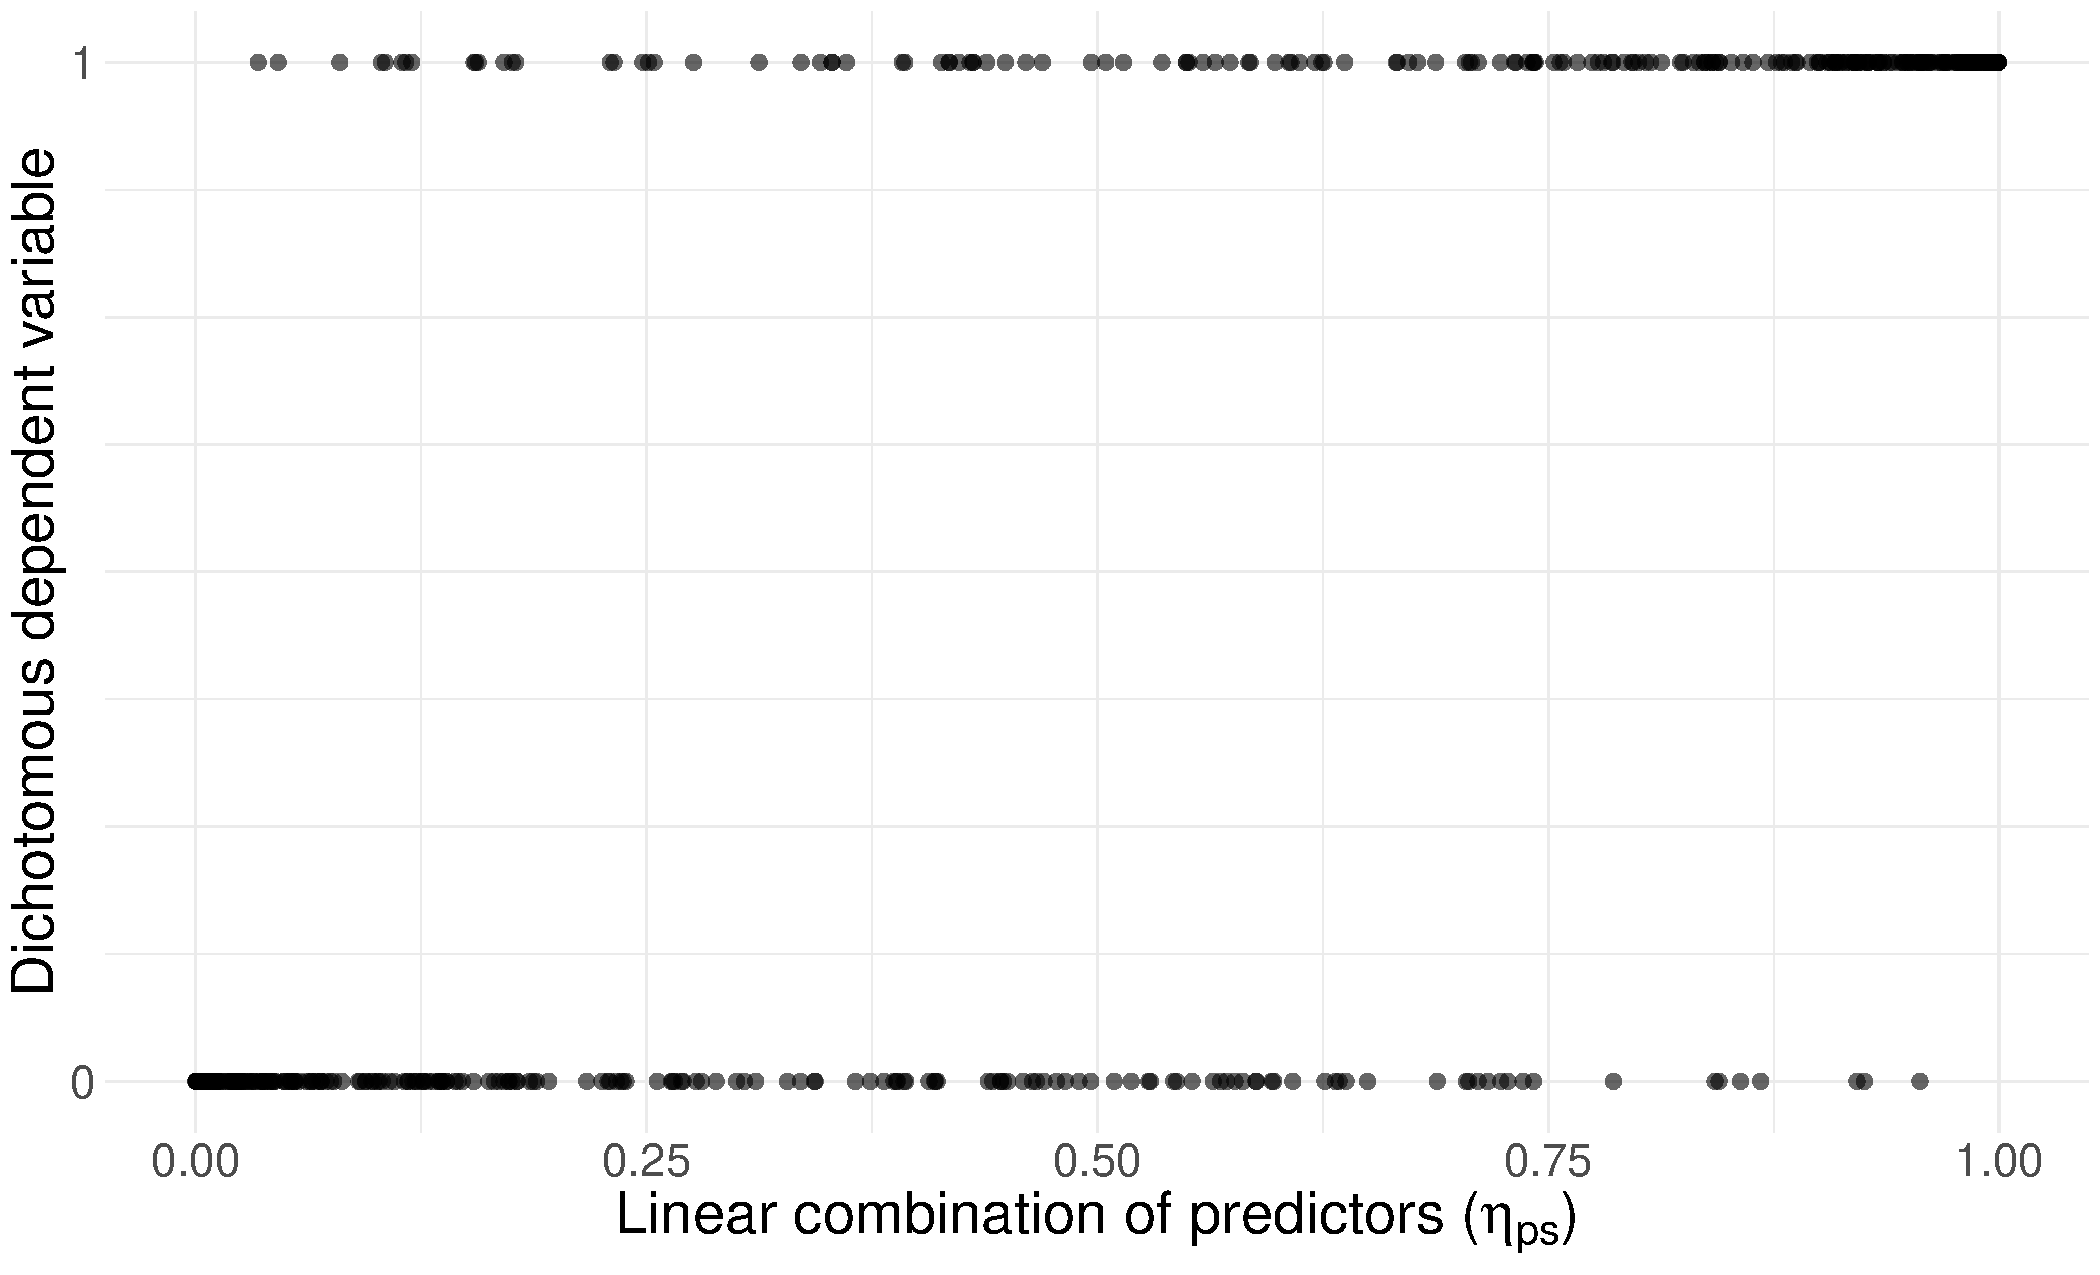
\includegraphics[width=0.7\linewidth]{img/baseGLM.pdf}
			\onslide<2>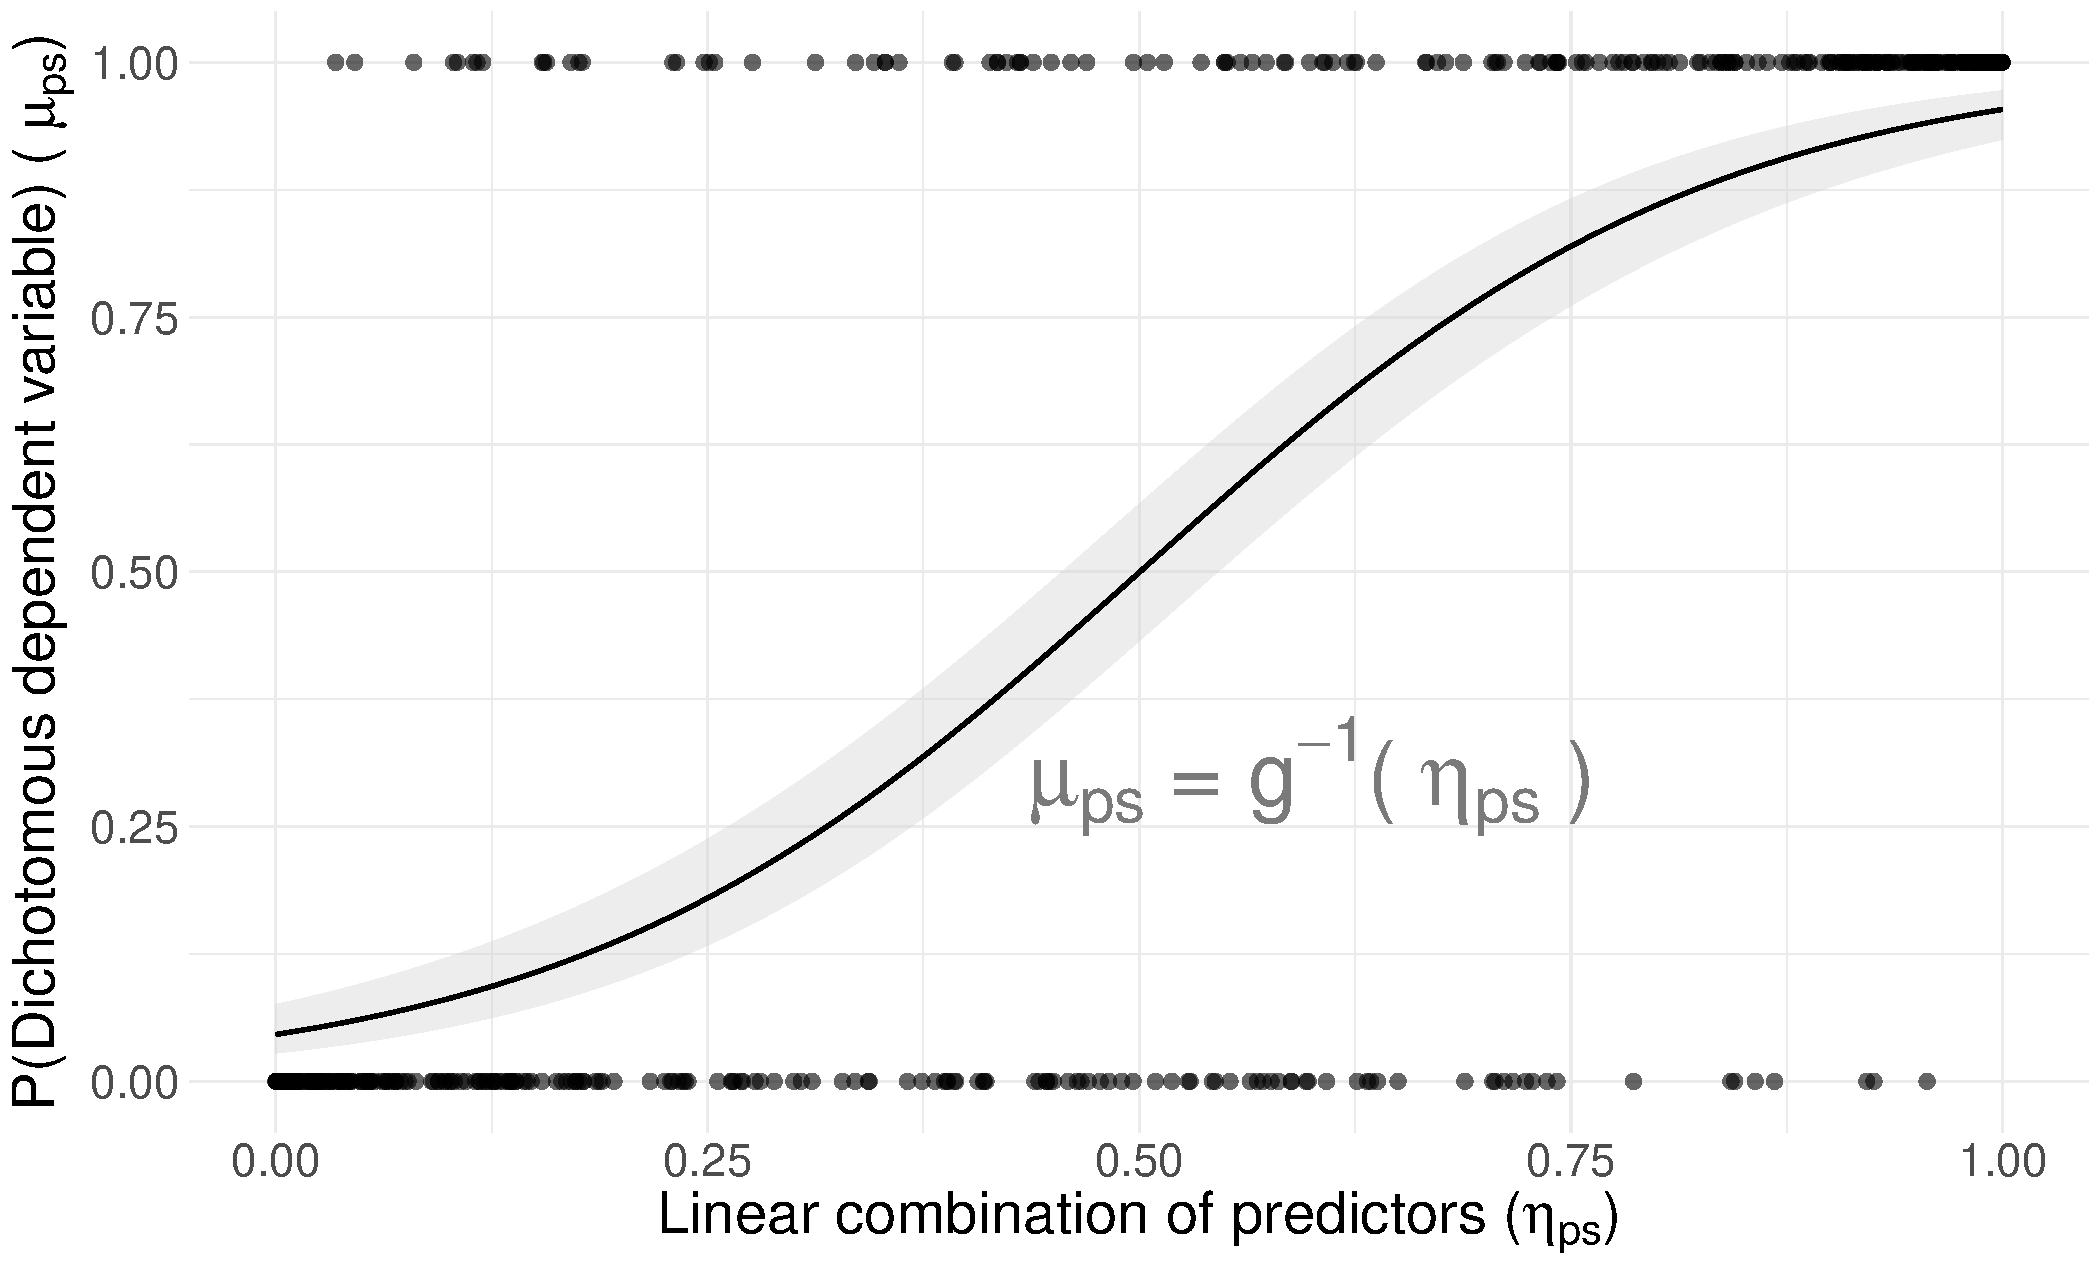
\includegraphics[width=0.7\linewidth]{img/linkGLM.pdf}
		\end{overprint}
	\end{figure}
	
	\onslide<2->
	\tikzoverlay (n1) at (8.5cm, 5.6cm){%
		\begin{minipage}{0.7\linewidth}
			
			Logit link function $g$:
			
			$g(\eta_{pi}) = log\left(\frac{\mu_{ps}}{1 - \mu_{ps}}\right)$
			
			\vspace{5mm}
			
			Inverse $g^{-1}$
			
			\vspace{5mm}
			
			$g^{-1} = \frac{\exp(\eta_{ps})}{1 + \exp(\eta_{ps})} $
			
			\vspace{1.5mm}
			%	where $\eta_{ps} = \theta_p + b_s$
		\end{minipage}
	}; 
	
\end{frame}

\subsection{Variabili latenti }

\begin{frame}{Il modello di Rasch}
	\begin{equation*}
		P(x_{ps} = 1| \theta_p, b_s) = \dfrac{\exp( \theta_p - b_s)}{1 + \exp(\theta_p - b_s)}
	\end{equation*}
	
	$\theta_p$: Abilità del soggetto $p$ \\
	$b_s$: difficoltà dello stimolo $s$\\
	
	\vspace{2.5mm}
	\onslide<2-> 
	\begin{columns}[T] % align columns
		\begin{column}{.50\linewidth}
			\textcolor{diff}{\rule{\linewidth}{2pt}}
			\begin{center}
				\textcolor{diff}{	\large{{Standard}}}
			\end{center}
			
		\end{column}
		
		\hfill%
		\begin{column}{.50\linewidth}
			\textcolor{single}{\rule{\linewidth}{2pt}}
			\begin{center}
				\textcolor{single}{\large{{GLM}}}	
			\end{center}
			
		\end{column}%
	\end{columns}
	
	\vspace{2.5mm}
	\begin{columns}[T]
		\begin{column}{.50\linewidth}
			\vspace*{2.5mm}
			$P(x_{ps} = 1) = \displaystyle \frac{\exp(\theta_p \spot<3-3>[fill=rasch!50]{-} b_s)}{1 + \exp(\theta_p \spot<3-3>[fill=rasch!50]{-} b_s)}$
		\end{column}
		\hfill
		
		\begin{column}{.50\linewidth}
			
			\vspace*{2.5mm}
			$P(x_{ps} = 1) = \displaystyle \frac{\exp(\theta_p \, \spot<3-3>[fill=single!50]{+} \, b_s)}{1 + \exp(\theta_p \, \spot<3-3>[fill=single!50]{+} \, b_s)}$
		\end{column}
	\end{columns}	
	
\end{frame}


\begin{frame}{E i tempi di risposta?}
	\begin{center}
		\Large\textcolor{log}{Modello log-normale}
	\end{center}
	
	
	\begin{columns}[T]
		\begin{column}{.50\linewidth}
						\textcolor{log}{\rule{\linewidth}{2pt}}
			\begin{center}
				\textcolor{log}{	\large{{Standard}}}
			\end{center}
			\centering
			$f (t_{ps}) =  \delta_s \, \spot<2-2>[fill=log!50]{-} \, \tau_p \, + \, \varepsilon $
		\end{column}
		\hfill
		
		\begin{column}{.50\linewidth}
				\textcolor{single}{\rule{\linewidth}{2pt}}
			\begin{center}
				\textcolor{single}{\large{{LM}}}	
			\end{center}
			\centering
			$f(t_{ps}) =  \delta_s \, \spot<2-2>[fill=single!50]{+} \, \tau_p \, +  \, \varepsilon$
		\end{column}
	\end{columns}	
	
	\vspace{3mm}
	$\tau_p$: Velocità del soggetto $p$ \\
	$\delta_s$: Time intensity dello stimolo $s$\\
	
	
	\vspace{3mm}
	\begin{alertblock}{N.B.}
		
		I tempi di risposta vanno log-trasformati
	\end{alertblock}
\end{frame}

%\begin{frame}{Alcuni dei problemi}
%	\begin{itemize}
%		\item La presenza di diversi scoring senza alcuna indicazione su quale usare e quando 
%		\item La presentazione del feedback 
%	\end{itemize}
%\end{frame}

\subsection*{Strutture random utili}

\begin{frame}
	\begin{footnotesize}
		La risposta attesa $y$ per l'osservazione $i = 1, \ldots, I$ del rispondente $p = 1,\ldots, P$ allo stimolo $s = 1,\ldots, S$ nella condizione $c= 1,\ldots, C$:
	\end{footnotesize}
	\footnotesize
	
	\vspace{3mm}
	Modello 1:
	\begin{equation*}\label{AccuracyMin}
		y_{i} = \spot[fill =blue!15]{\alpha + \beta_c X_c}  + \spot[fill=yellow!20]{\alpha_{p[i]} +  \alpha_{s[i]} + \varepsilon_{i}}
	\end{equation*}
	\begin{centering}
		
		$\alpha_p \sim \mathcal{N}(0, \sigma_p^2)$,
		
	\end{centering}
	
	\begin{centering}
		
		$\alpha_s \sim \mathcal{N}(0, \sigma_s^2)$.
		
	\end{centering}
	
	
	
	Modello 2: 
	\begin{equation*}\label{Accuracy5}
		y_{i} = \spot[fill =blue!15]{\alpha + \beta_c X_c}  + \spot[fill=yellow!20]{ \alpha_{p[i]} +  \beta_{s[i]}c_{i} + \varepsilon_{i}}
	\end{equation*}
	
	\begin{centering}
		$\alpha_p \sim \mathcal{N}(0, \sigma_p^2)$,
		
	\end{centering}
	
	\begin{centering}
		
		$\beta_s \sim \mathcal{MVN}(0, \Sigma_{sc})$.
		
	\end{centering}
	
	Modello 3: 
	
	\begin{equation*}
		y_{i} = \spot[fill =blue!15]{\alpha + \beta_c X_c}  + \spot[fill=yellow!20]{\alpha_{s[i]} +  \beta_{p[i]}c_{i} + \varepsilon_{i}}
	\end{equation*}
	
	\begin{centering}
		$\alpha_s \sim \mathcal{N}(0, \sigma_s^2)$,
		
	\end{centering}
	
	\begin{centering}
		
		$\beta_p \sim \mathcal{MVN}(0, \Sigma_{pc})$.
		
	\end{centering}
	
	
	\vspace{3mm}
	
	\footnotesize{Accuratezza: $\epsilon \sim Logistic (0, \sigma^2)$ \\ Log-tempi: $\epsilon \sim \mathcal{N} (0, \sigma^2)$}
	
	
	
	%	\only<2->{
		\begin{textblock*}{10cm}(10cm,3cm)
			\spot(last)[fill = blue!15]{Effetti Fissi}
		\end{textblock*}
		%}
	\begin{textblock*}{10cm}(9.5cm,5cm)
		\spot(last)[fill = yellow!20]{Effetti random}
	\end{textblock*}
\end{frame}

\begin{frame}{Parametrizzazioni}
	\vspace{5mm}
	{\textcolor{rasch}{\textbf{Modelli sulle accuratezza (stime simil Rasch):}}}
	\vspace{2mm}
	\begin{table}
		\centering
		\begin{tabular}{l l l}
			\hline
			& \textbf{Respondent} & \textbf{Stimulus}\\
			\hline				
			
			Model 1  & 	 Overall ($\theta_p$) & Overall ($b_s$) \\		
			Model 2 & Overall ($\theta_p$) & Condition--specific ($b_{sc}$)\\
			Model 3 &Condition--specific ($\theta_{pc}$)  & Overall ($b_s)$ \\
			\hline
		\end{tabular}
	\end{table}
	
	\vspace{3mm}
	{\textcolor{log}{{\textbf{Modelli sui log-tempi (stime del modello log-normale):}}}}
	\vspace{2mm}
	\begin{table}
		\centering
		\begin{tabular}{l l l}
			\hline
			& \textbf{Respondent} & \textbf{Stimulus}\\
			\hline					 
			Model 1  & Overall  ($\tau_p$) & Overall ($\delta_s)$ \\	
			Model 2 & Overall ($\tau_p$) & Condition--specific ($\delta_{sc})$ \\
			Model 3 & Condition--specific ($\tau_{pc}$) & Overall ($\delta_s)$ \\
			\hline
		\end{tabular}
	\end{table}
\end{frame}

\section{In pratica}

\subsection{Step preparativi}
\begin{frame}[fragile]
	Questi modelli possono essere stimati in \texttt{R} con il pacchetto \texttt{lme4}
	
	\begin{lstlisting}
install.packages(``lme4'') # per stimare i modelli
install.packages(``ggplot2'') # per fare i grafici
install.packages(``car'') # per preprocessing
library(lme4)
library(ggplot2)
	\end{lstlisting}

Il data set su cui faremo questa esercitazione è disponibile a questa pagina: \href{https://ottaviae.github.io/DscoreApp/}{https://ottaviae.github.io/DscoreApp/} (Sottosezione ``Data''). Possono essere importati usando questo codice
	
\begin{lstlisting}
my_url = "https://ottaviae.github.io/DscoreApp/raceAPP.csv"
iat_data = read.csv(url(my_url))

\end{lstlisting}
\end{frame}

\begin{frame}[fragile]{Un po' di ordine}

\begin{lstlisting}
# sistema l'etichetta di uno stimolo 
temp = iat_data[iat_data$stimoli %in% "felicit\xe0", ]
iat_data = iat_data[!iat_data$stimoli %in% "felicit\xe0", ]
temp$stimoli = "felic"
iat_data = rbind(iat_data, temp)

# seleziona solo le colonne su cui facciamo le analisi
iat_data = iat_data[, c("participant", "blockcode", "stimoli", "latency", "correct")]
# rinomina le colonne in modo che siano uguali per tutt3
colnames(iat_data)[2:3] = c("condition", "stimuli")
# rinomina le condizioni
iat_data$condition = car::recode(iat_data$condition,
"'Whitegood' = 'WGBB';
'Whitebad' = 'BGWB'")
\end{lstlisting}

\end{frame}

\subsection{Stima dei modelli}

\begin{frame}[fragile]{Modello 1}

	\begin{equation*}
	y_{i} = {\alpha + \beta_c X_c}  + {\alpha_{p[i]} +  \alpha_{s[i]} + \varepsilon_{i}}
\end{equation*}

Accuratezze: 

\begin{lstlisting}
iat_accuracy1 = glmer(correct ~ 0 + condition  + (1|participant) + 
	(1|stimuli),
	data = iat_data,
	family = "binomial")
\end{lstlisting}

Log-tempi:


\begin{lstlisting}
iat_time1 = lmer(log(latency) ~ 0 + condition + (1|participant) + 
	(1|stimuli),
	REML = FALSE,
	data = iat_data)
	summary(iat_time1)
\end{lstlisting}

\end{frame}

\begin{frame}[fragile]{Modello 2}
	
	\begin{equation*}
	y_{i} = {\alpha + \beta_c X_c}  + { \alpha_{p[i]} +  \beta_{s[i]}c_{i} + \varepsilon_{i}}
	\end{equation*}
	
	Accuratezze: 
	
	\begin{lstlisting}
iat_accuracy2 = glmer(correct ~ 0 + condition + (1|participant) + 
	(0 + condition|stimuli),
	data = iat_data,
	family = "binomial")
	\end{lstlisting}
	
	Log-tempi:
	
	
	\begin{lstlisting}
iat_time2 = lmer(log(latency) ~ 0 + condition + (1|participant) + 
	(0 + condition |stimuli),
	REML = FALSE,
	data = iat_data)
	\end{lstlisting}
	
\end{frame}
%
%
\begin{frame}[fragile]{Modello 3}
	
	\begin{equation*}
	y_{i} = {\alpha + \beta_c X_c}  + {\alpha_{s[i]} +  \beta_{p[i]}c_{i} + \varepsilon_{i}}
	\end{equation*}
	
	Accuratezze: 
	
	\begin{lstlisting}
iat_accuracy3 = glmer(correct ~ 0 + condition + 
	(0 + condition|participant) + (1|stimuli),
	data = iat_data,
	family = "binomial")
	\end{lstlisting}
	
	Log-tempi:
	
	
	\begin{lstlisting}
iat_time3 = lmer(log(latency) ~ 0 + condition + 
	(0 + condition |participant) + (1|stimuli),
	REML = FALSE,
	data = iat_data)
	\end{lstlisting}
	
\end{frame}

\subsection{Model comparison}

\begin{frame}[fragile]{Accuratezze}

\begin{lstlisting}
anova(iat_accuracy1, iat_accuracy2, iat_accuracy3)
\end{lstlisting}

\begin{figure}
	\centering
	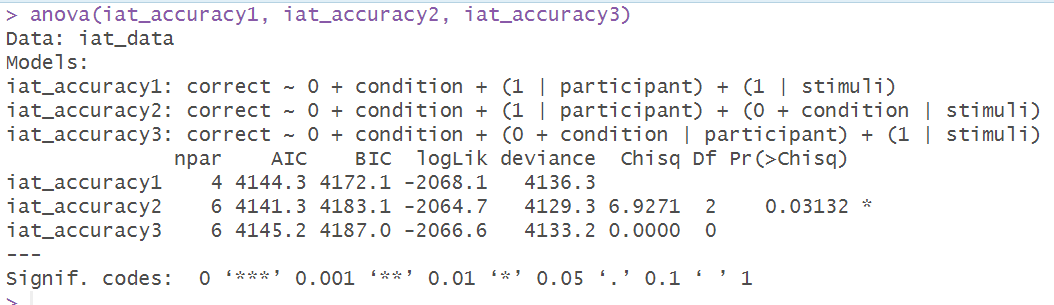
\includegraphics[width=\linewidth]{anova-accuracy}
\end{figure}
\end{frame}

\begin{frame}[fragile]{The winner is...}
	\vspace*{-5.6mm}
\begin{figure}
	\centering
	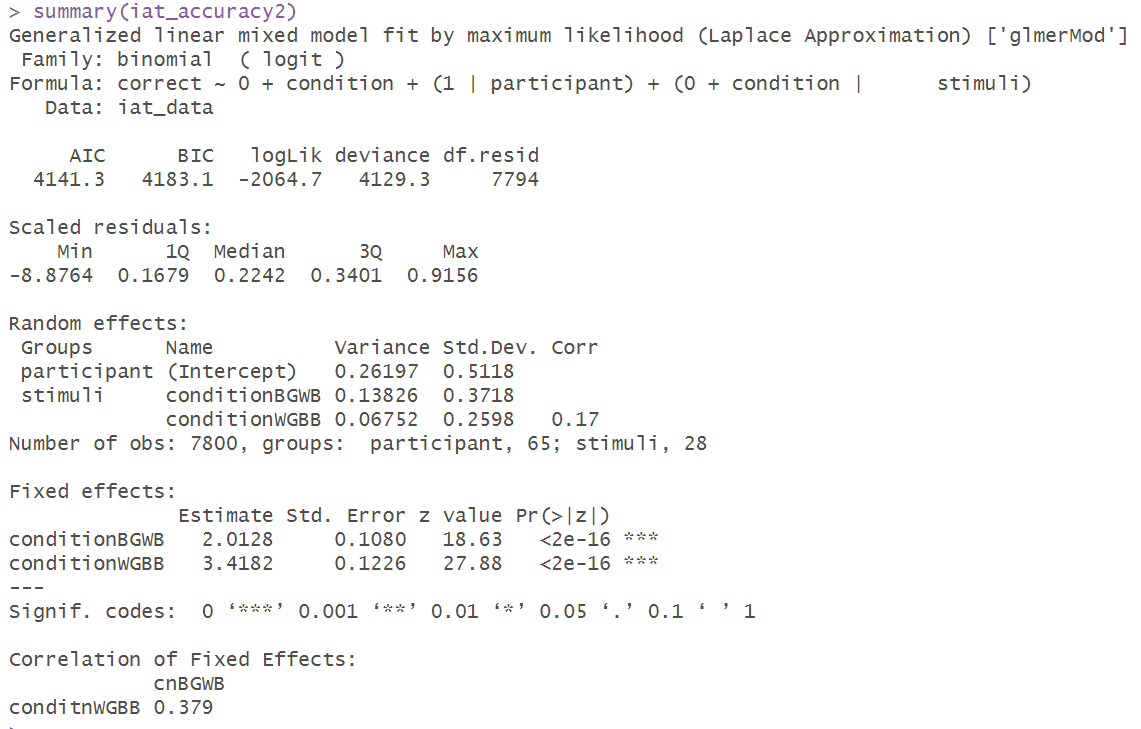
\includegraphics[width=.8\linewidth]{accuracym2}
\end{figure}
	
	\begin{footnotesize}
		Per ottenere le proporzioni di risposte corrette nelle due condizioni: 
\begin{lstlisting}
exp(fixef(iat_accuracy2))/(1 + exp(fixef(iat_accuracy2)))
\end{lstlisting}
	\end{footnotesize}

\end{frame}

\begin{frame}[fragile]{Log-tempi}
	\begin{lstlisting}
		anova(iat_time1, iat_time2, iat_time3)
	\end{lstlisting}
	
	
	\begin{figure}
		\centering
		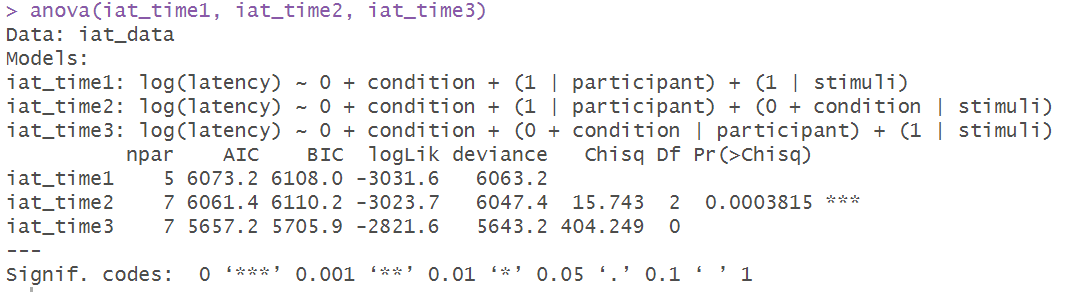
\includegraphics[width=\linewidth]{anova-time1}
	\end{figure}
	
	Attenzione! Il modello 2 non arriva a convergere
\end{frame}

\begin{frame}{And the winner is...}
	\vspace*{-5.6mm}
	\begin{figure}
		\centering
		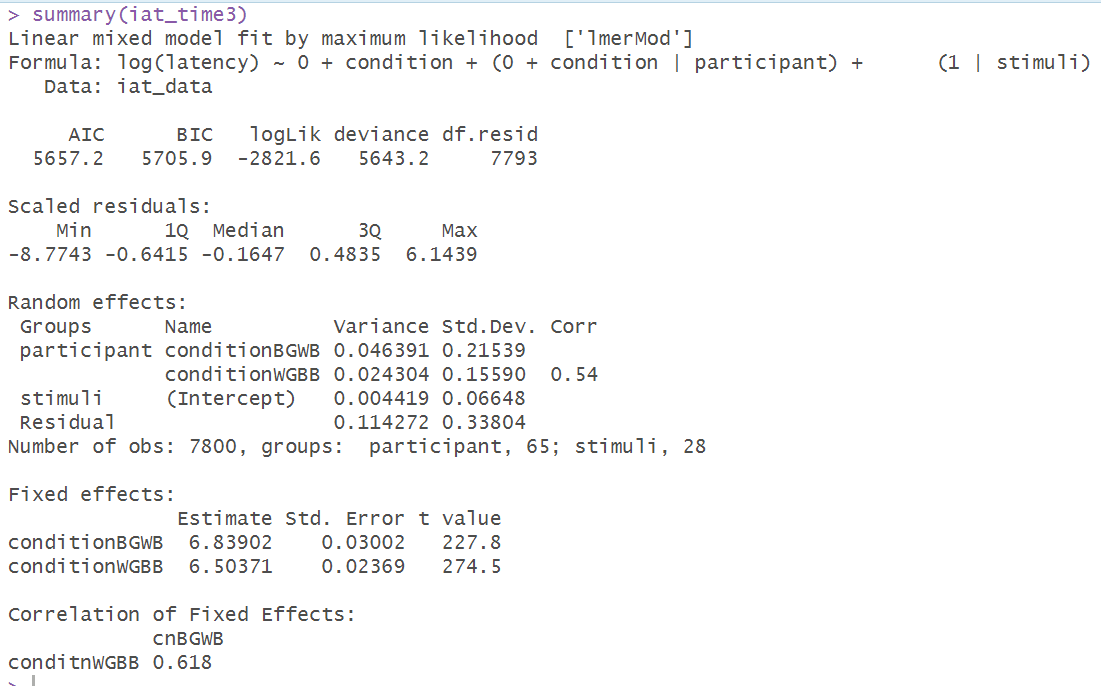
\includegraphics[width=.95\linewidth]{accuracyt3}
	\end{figure}
	
\end{frame}

\subsection{Estrarre le stime del modello vincente}

\begin{frame}[fragile]{Accuratezze}
	
	Abilità dei soggetti $\theta_p$: 
\begin{small}
		\begin{lstlisting}
ab_iat = data.frame(sbj = rownames(coef(iat_accuracy2)$participant), 
		theta = coef(iat_accuracy2)$participant[,1]) 
# grafico
graph_theta_iat = ggplot(ab_iat, 
			aes(x = theta)) +  geom_density() 	
graph_theta_iat  
		\end{lstlisting}
\end{small}


\begin{figure}
	\centering
	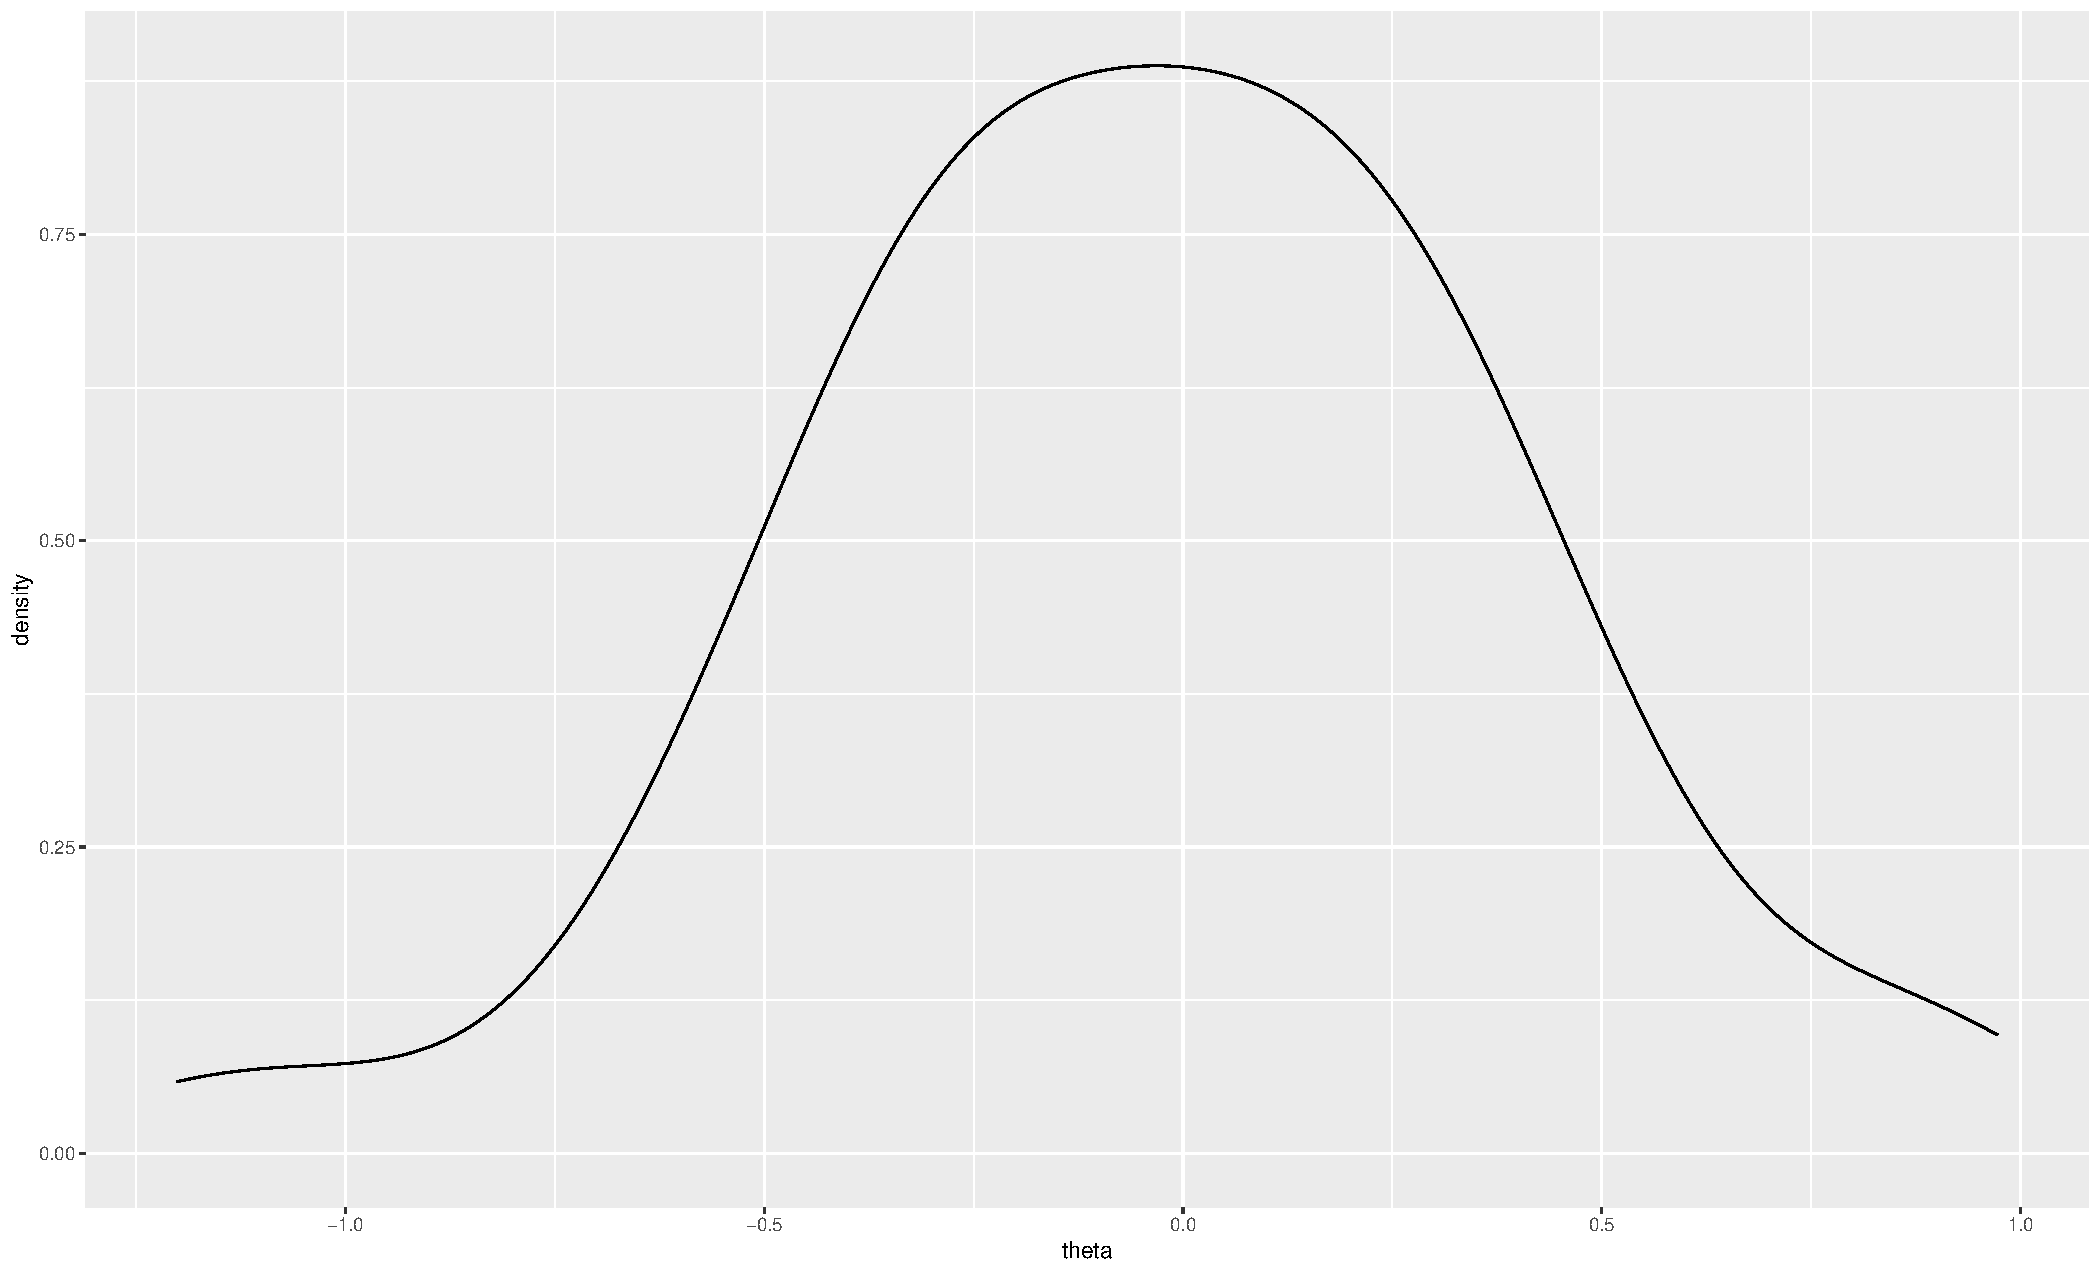
\includegraphics[width=.5\linewidth]{ability-IAT}
\end{figure}

\end{frame}

\begin{frame}[fragile]{Accuratezze}
	
Difficoltà degli item condizione--specifica $b_{sc}$
	\begin{lstlisting}
# effetti random con dev std
blup_easiness_iat = as.data.frame(ranef(iat_accuracy2,   
		condVar = TRUE))
# effetti fissi
fixef_accuracy_iat = data.frame(term = names(fixef(iat_accuracy2)), 
			est = (fixef(iat_accuracy2))) 
# unire effetti fissi ed effetti random
easiness_iat = merge(blup_easiness_iat, fixef_accuracy_iat)
colnames(easiness_iat) = c("Condition", "grpvar", "stimuli",
"blup", "se", "fix.est")
# calcola parametro dell'item
easiness_iat$b = with(easiness_iat, fix.est + blup)
	\end{lstlisting}
	
\end{frame}

\begin{frame}[fragile]{Il plot}

	\begin{lstlisting}
graph_b_ci = ggplot(easiness_iat, 
	aes(x = b, 	y = stimuli,  color = Condition)) + 
	geom_point() +
	geom_errorbarh(aes(xmin = b - 1.96*se, 
				xmax= b + 1.96*se))
graph_b_ci 
\end{lstlisting}



\end{frame}


\begin{frame}
		
	\begin{figure}
		\centering 
		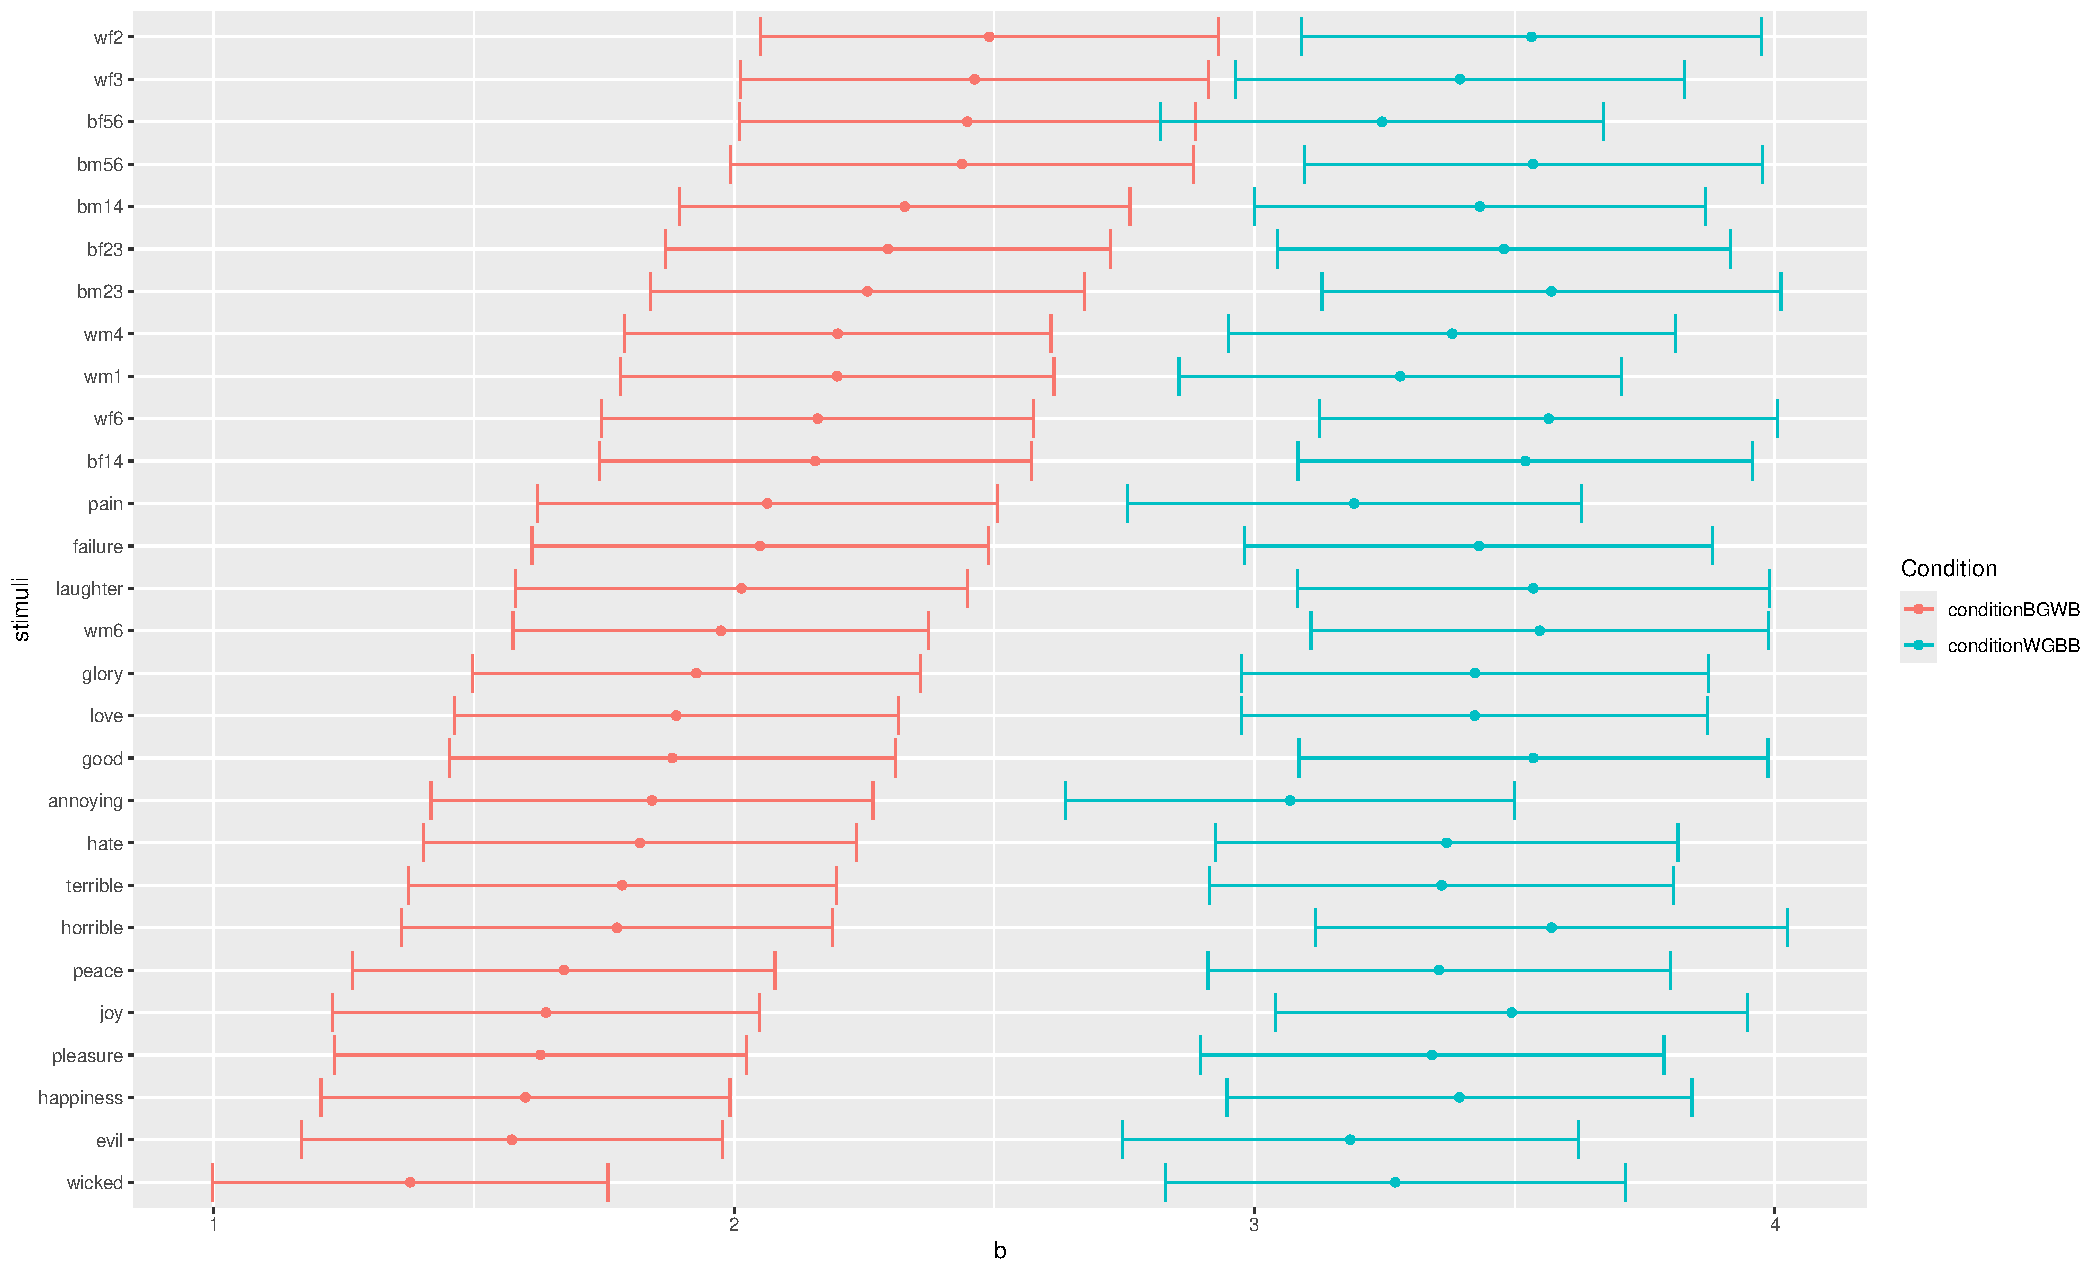
\includegraphics[width=\linewidth]{easy-IAT}
	\end{figure}
\end{frame}


\begin{frame}[fragile]{Log-tempi}
	
	Velocità dei soggetti condizione--specifica $\tau_{pc}$
	\begin{lstlisting}
speed_iat = coef(iat_time3)$participant[,-1] 
# formato long
sp_iat = stack(speed_iat)
# rinomina le colonne
colnames(sp_iat) = c("tau", "condition")
graph_speed_iat = ggplot(sp_iat,
	aes(x = tau, fill = condition)) + geom_density() 
	\end{lstlisting}

	
\end{frame}


\begin{frame}{Il risultato}
	\begin{figure}
	\centering 
	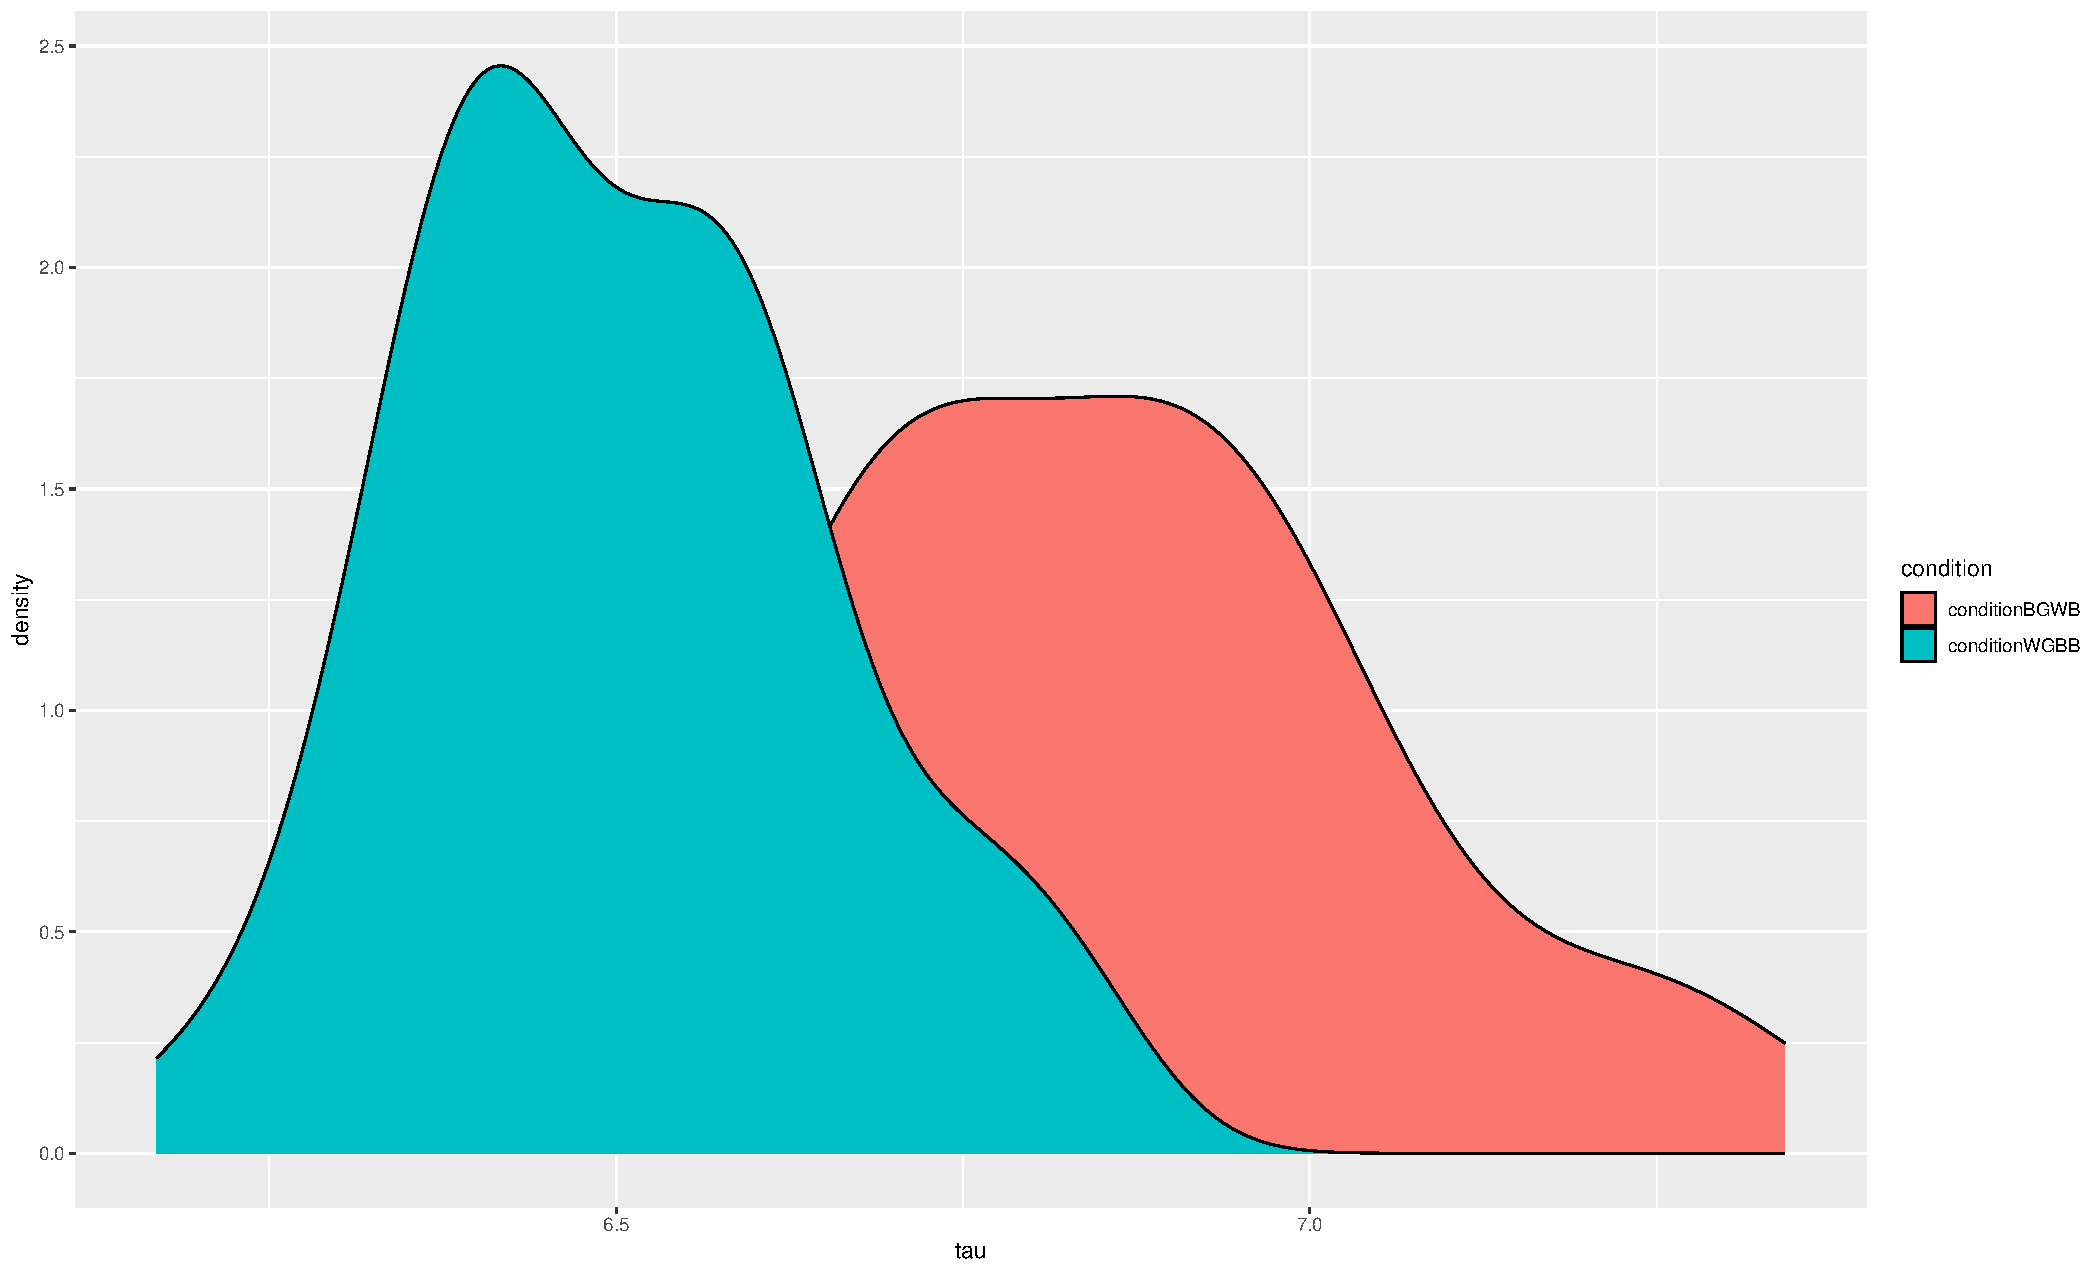
\includegraphics[width=.90\linewidth]{speed-IAT}
\end{figure}
\end{frame}

\begin{frame}[fragile]{Log-tempi}
	
	Time intensity degli item $\delta_s$:
	

	\small
\begin{lstlisting}
intensity_iat = data.frame(
		stimulus = rownames(coef(iat_time3)$stimuli), 
		intensity = coef(iat_time3)$stimuli[,1]) 
graph_delta_iat = ggplot(intensity_iat, 
		(aes(x = intensity, y = stimulus))) +  geom_point() 
graph_delta_iat 

\end{lstlisting}
	
	\begin{figure}
		\centering
		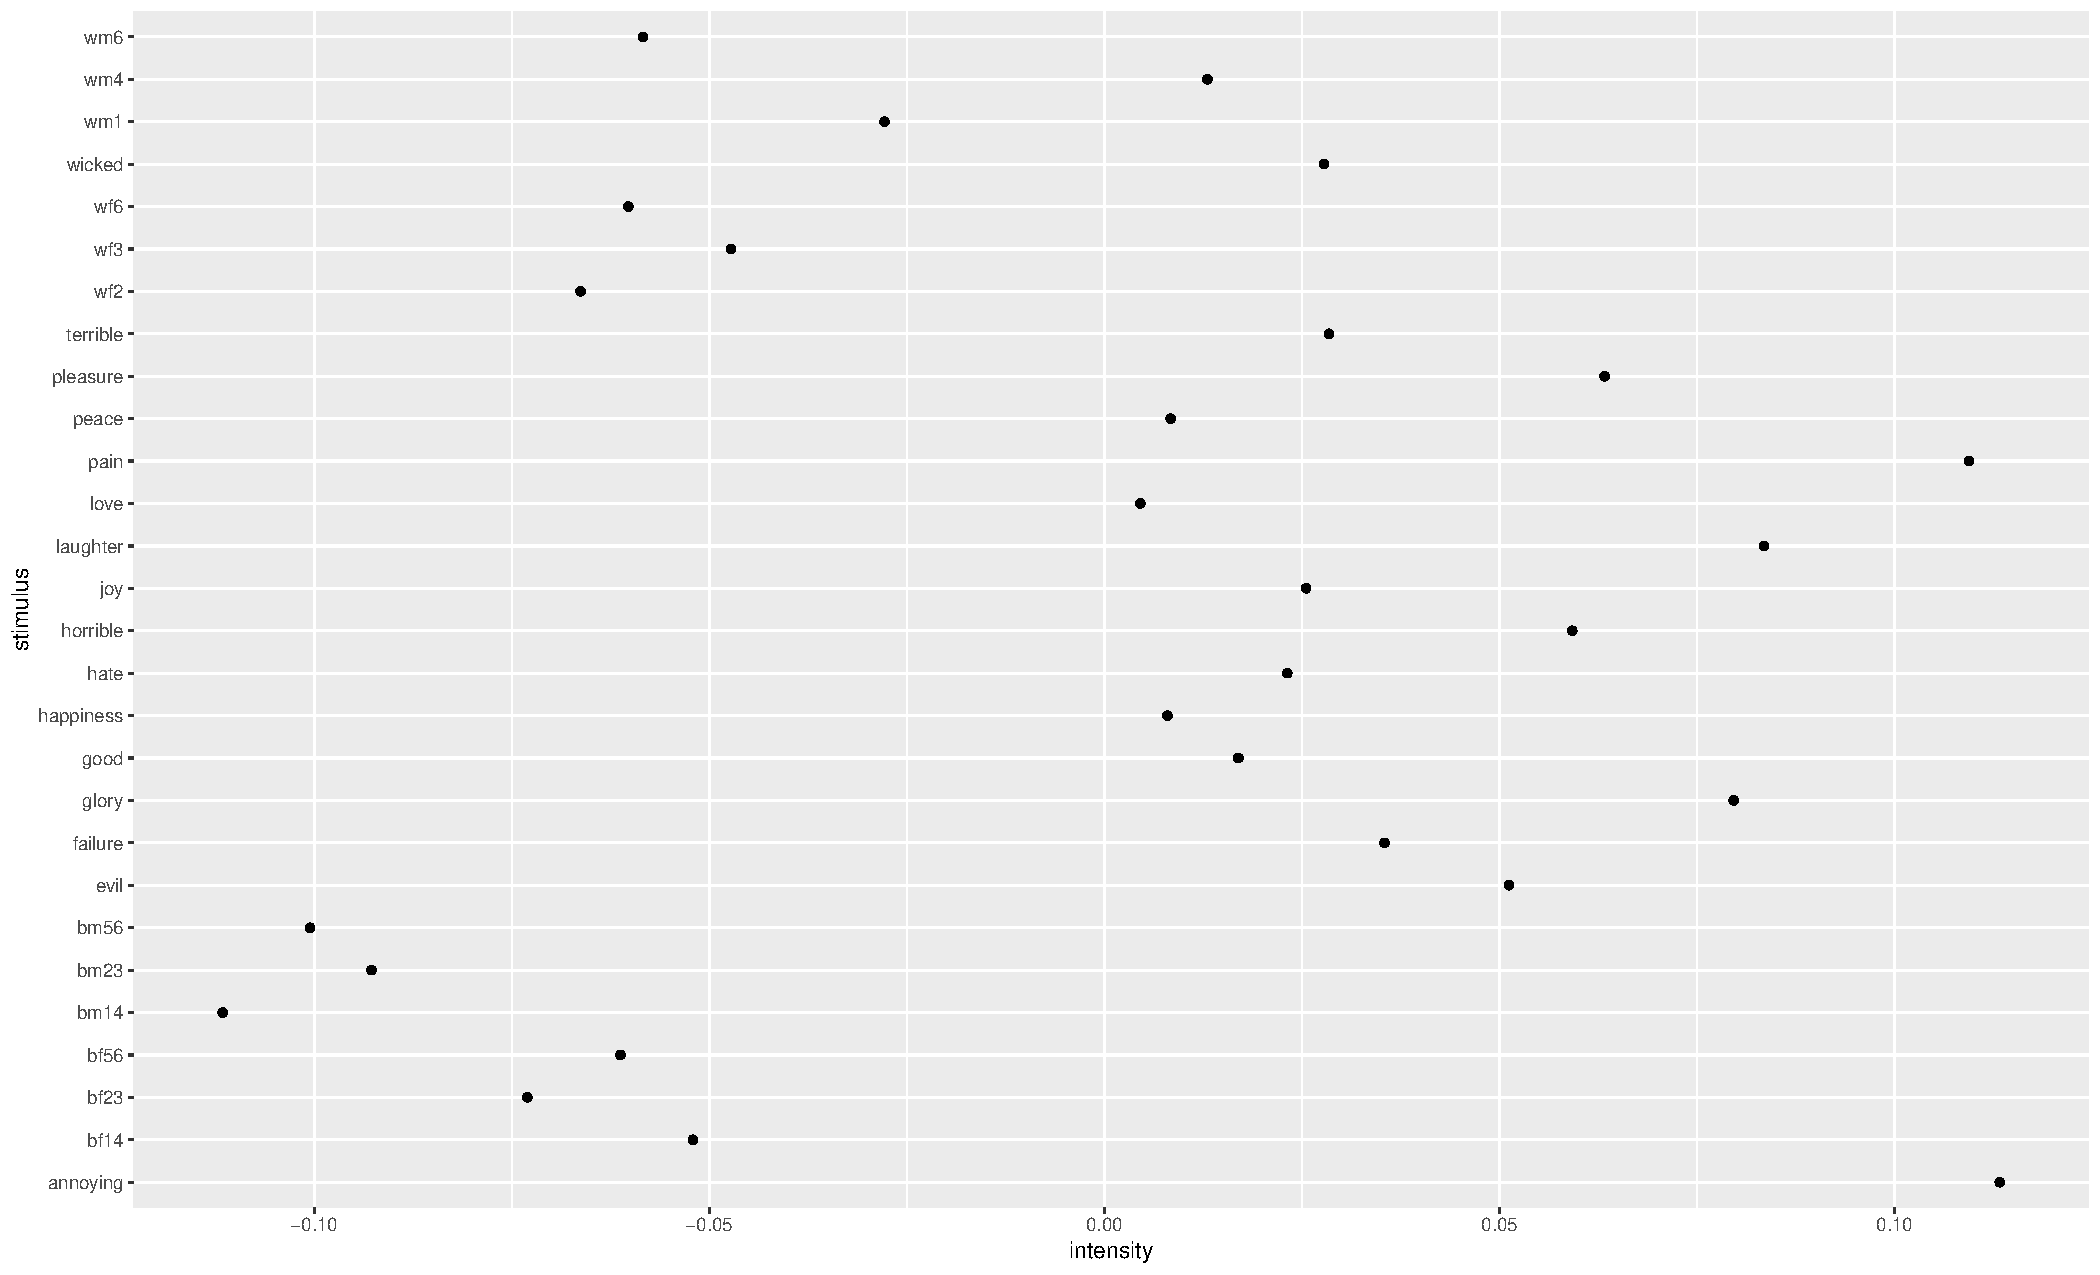
\includegraphics[width=.5\linewidth]{intensity-IAT}
	\end{figure}
	
\end{frame}


\end{document}